% 開発環境


%%%%%%%%%%%%%%%%%%%%%%%%%%%%%%%%%%%%%%%%%%%%%%%%

\section{概要}
本章では,本研究において使用した開発環境および機器について述べる。
本研究では,新規に試作した携帯型CO$_2$測定デバイスを中心に,マイクロコントローラ,センサ,通信モジュール,電源系を含むハードウェア構成を設計・実装した。
また,性能比較および有効性検証のため,先行研究で使用された機器についても併せて説明する。

\section{新規に作成した機器}
本研究では,携帯型CO$_2$測定デバイスの実現を目的として,新たにハードウェア構成を設計・試作した。
本節では,試作機を構成する各機器について説明する。

\subsection{マイクロコントローラ ESP32-C6}
本研究では,マイクロコントローラとして Seeed Studio XIAO ESP32-C6 を採用した。
本モジュールは ESP32-C6 SoC を搭載しており,2つの32ビット RISC-V プロセッサで構成されている。
高性能(High Performance: HP)プロセッサは最大160\,MHzで動作し,低消費電力(Low Power: LP)プロセッサは最大20\,MHzでの動作が可能である。

また,512\,KBのSRAMおよび4\,MBのフラッシュメモリを内蔵しており,センサ制御,通信処理,データ管理を同時に行うIoT用途に十分な記憶容量を備えている。
無線通信機能として,2.4\,GHz Wi-Fi 6,Bluetooth 5.3,Zigbee,Thread(IEEE 802.15.4)をサポートしており,Matterにネイティブ対応している点も特徴である。

これらの特性から,本研究では高い演算性能と低消費電力動作を両立できるマイクロコントローラとして ESP32-C6 を採用した。

\begin{figure}[H]
\centering

\begin{minipage}{0.42\linewidth}
  \centering
  \includegraphics[width=\linewidth]{./figures/SeeedESP32C6}
  \captionof{figure}{SeeedESP32C6}
  \label{fig:SeeedESP32C6}
\end{minipage}
\hfill
\begin{minipage}{0.52\linewidth}
  \centering
  \captionof{table}{ESP32C6の主なパラメータ}
  \label{tab:scd41Parameters}
  \begin{tabular}{|c|c|}
    \hline
    モデルNo. & SCD41 \\ \hline \hline
    I2Cアドレス & 0x62 \\ \hline
    測定対象 & CO$_2$,温度,湿度 \\ \hline
    CO$_2$測定範囲 & 400$\sim$5000 ppm \\ \hline
    CO$_2$測定精度 & $\pm$(40 ppm + 5\%) \\ \hline
    温度測定範囲 & -10$\sim$60 ℃ \\ \hline
    湿度測定範囲 & 0$\sim$95 \%RH \\ \hline
    解像度 & 16ビット \\ \hline
    入力電圧 & 2.4$\sim$5.5 V \\ \hline
    平均消費電流 & 約15 mA \\ \hline
    ボード寸法 & 約10.1 $\times$ 10.1 $\times$ 7.0 mm \\ \hline
    対応温度 & -10$\sim$60 ℃ \\ \hline
  \end{tabular}
\end{minipage}

\end{figure}


\FloatBarrier


\subsection{CO$_2$センサモジュール SCD41}
二酸化炭素濃度は,室内空気質を評価する上で重要な指標の一つであり,換気状態や居住環境の快適性と密接に関係している。
本研究では,CO$_2$センサとして Sensirion 社製 SCD41 を搭載したモジュールを使用した。

SCD41 は NDIR(Non-Dispersive Infrared)方式を採用した高精度なCO$_2$センサであり,小型かつ低消費電力である点が特徴である。
また,温度および湿度センサを内蔵しており,これらの測定値を用いた補正により,安定したCO$_2$濃度測定が可能である。

本モジュールは 2.54\,mm ピッチのピンインターフェースを備えており,I$^2$C通信によってマイクロコントローラと接続される。
これにより,携帯型デバイスへの組み込みが容易であり,本研究の目的に適している。
本モジュールの主なパラメータを表\ref{tab:scd41Parameters}に示す。


\begin{figure}[H]
\centering

\begin{minipage}{0.42\linewidth}
  \centering
  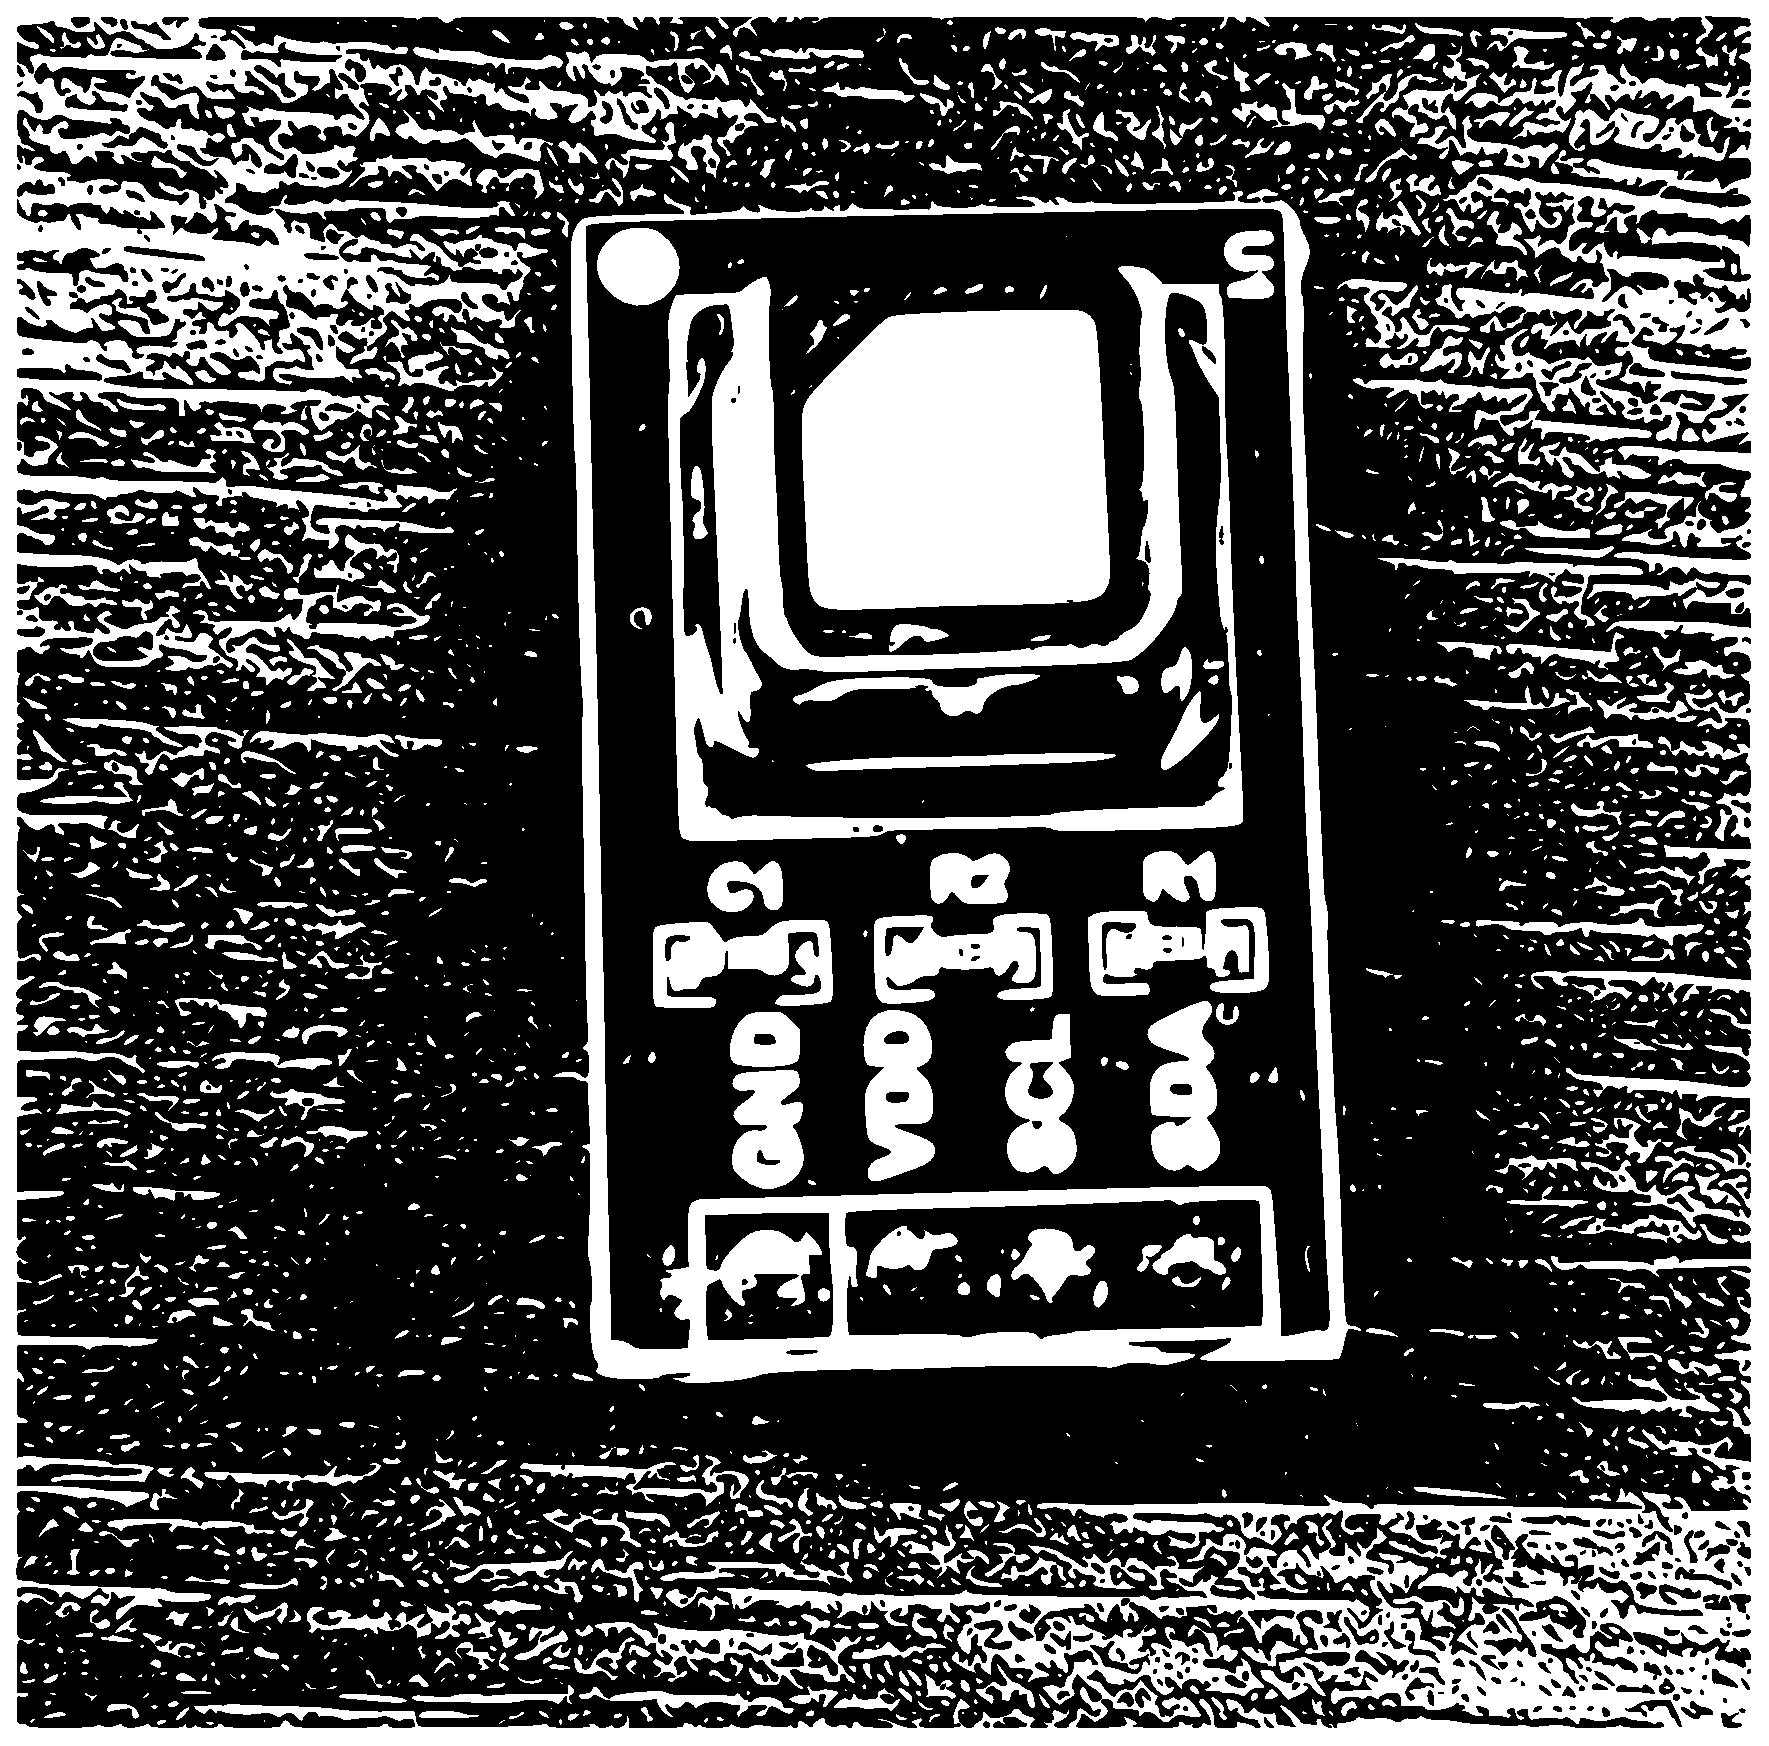
\includegraphics[width=\linewidth]{./figures/scd41_new}
  \captionof{figure}{SCD41}
  \label{fig:sensor}
\end{minipage}
\hfill
\begin{minipage}{0.52\linewidth}
  \centering
  \captionof{table}{SCD41の主なパラメータ}
  \label{tab:scd41Parameters}
  \begin{tabular}{|c|c|}
    \hline
    モデルNo. & SCD41 \\ \hline \hline
    I2Cアドレス & 0x62 \\ \hline
    測定対象 & CO$_2$,温度,湿度 \\ \hline
    CO$_2$測定範囲 & 400$\sim$5000 ppm \\ \hline
    CO$_2$測定精度 & $\pm$(40 ppm + 5\%) \\ \hline
    温度測定範囲 & -10$\sim$60 ℃ \\ \hline
    湿度測定範囲 & 0$\sim$95 \%RH \\ \hline
    解像度 & 16ビット \\ \hline
    入力電圧 & 2.4$\sim$5.5 V \\ \hline
    平均消費電流 & 約15 mA \\ \hline
    ボード寸法 & 約10.1 $\times$ 10.1 $\times$ 7.0 mm \\ \hline
    対応温度 & -10$\sim$60 ℃ \\ \hline
  \end{tabular}
\end{minipage}

\end{figure}

\FloatBarrier

\subsection{リチウムポリマバッテリ}
本研究で試作した携帯型CO$_2$測定デバイスの電源として,リチウムポリマバッテリを使用した。
リチウムポリマバッテリは,高エネルギー密度,小型・軽量である点から,携帯機器やウェアラブルデバイスに広く利用されている。

本研究では,長時間駆動および携帯性の両立を目的として,バッテリ駆動による動作を前提とした設計を行った。

\subsection{LTE通信モジュール SIM7080G}
通信モジュールとして,SIMCom 社製 SIM7080G を使用した。
SIM7080G は,LTE Cat.M1 および NB-IoT に対応した低消費電力通信モジュールであり,M2M および IoT 用途に特化して設計されている。

本モジュールは Qualcomm 製コアを搭載し,省電力クラス Class~5 に対応している。
また,グローバルモデルであるため,幅広い通信環境での利用が可能である。
本研究では,屋外や移動環境においても測定データをサーバへ送信することを目的として,本モジュールを採用した。
本モジュールの主なパラメータを表\ref{tab:sim7080gParameters}に示す。

\begin{figure}[H]
\centering

\begin{minipage}{0.42\linewidth}
  \centering
  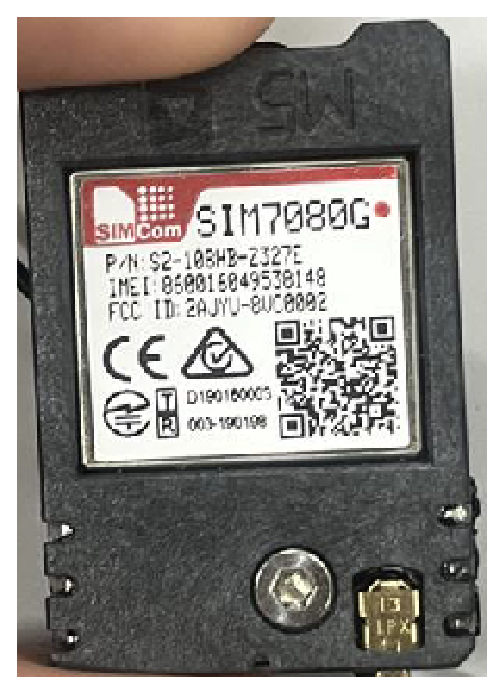
\includegraphics[width=\linewidth]{./figures/porttype}
  \captionof{figure}{SIM7080G}
  \label{fig:SIM7080G}
\end{minipage}
\hfill
\begin{minipage}{0.52\linewidth}
  \centering
  \captionof{table}{SIM7080Gの主なパラメータ}
  \label{tab:sim7080gParameters}
  \begin{tabular}{|c|c|}
    \hline
    項目 & 内容 \\ \hline \hline
    対応通信方式 & LTE Cat.M1 / NB-IoT \\ \hline
    対応周波数帯 & LTE Band 1, 3, 8, 18, 19, 26 ほか \\ \hline
    通信プロトコル & TCP/IP, UDP, HTTP \\ \hline
    動作電圧 & 3.3$\sim$4.2 V \\ \hline
    消費電力(待機時) & 数 mA 程度 \\ \hline
    動作温度範囲 & -40$\sim$85 ℃ \\ \hline
    用途 & M2M / IoT 通信 \\ \hline
  \end{tabular}
\end{minipage}

\end{figure}
\FloatBarrier

\subsection{SIMカード}
本研究では,LTE 通信に IIJ(インターネットイニシアティブ)社が提供する SIM カードを使用した。
本 SIM カードを用いることで,SIM7080G を介したモバイル通信が可能となる。
これにより,設置場所に依存しないデータ収集が可能となり,携帯型測定デバイスとしての有効性を検証できる構成とした。

\section{先行研究で使用した機器}
本研究では,提案手法の有効性を検証するため,先行研究で使用された機器との比較を行った。
本節では,先行研究で用いられた主な機器について説明する。

\subsection{Arduino MKR WiFi 1010}
Arduino MKR WiFi 1010 は,SAMD21G18A マイクロコントローラを中心に,無線通信機能を担う NINA-W102 モジュールや,セキュア通信を実現する暗号チップ ATECC508 を搭載した小型開発ボードである。また,外部 SPI フラッシュメモリとして 2\,MB の記憶領域を備えており,プログラムやデータの保存が可能である。先行研究では,室内環境計測用デバイスの制御用マイクロコントローラとして使用されていた。

\begin{figure}[h]
\centering
\includegraphics[width=.5\linewidth]{./figures/Arduino}
\caption{Arduino MKR WiFi 1010}
\label{fig:Arduino}
\end{figure}
\FloatBarrier

\subsection{CO$_2$センサ MH-Z19C}
MH-Z19C は,Winsen 社が製造する NDIR 方式の CO$_2$ センサモジュールである。比較的安価であり,室内環境測定用途として広く利用されている。先行研究では,本センサを用いて CO$_2$ 濃度の測定が行われていた。本モジュールの主なパラメータを表\ref{tab:mhz19cParameters}に示す。

\begin{figure}[H]
\centering

\begin{minipage}{0.42\linewidth}
  \centering
  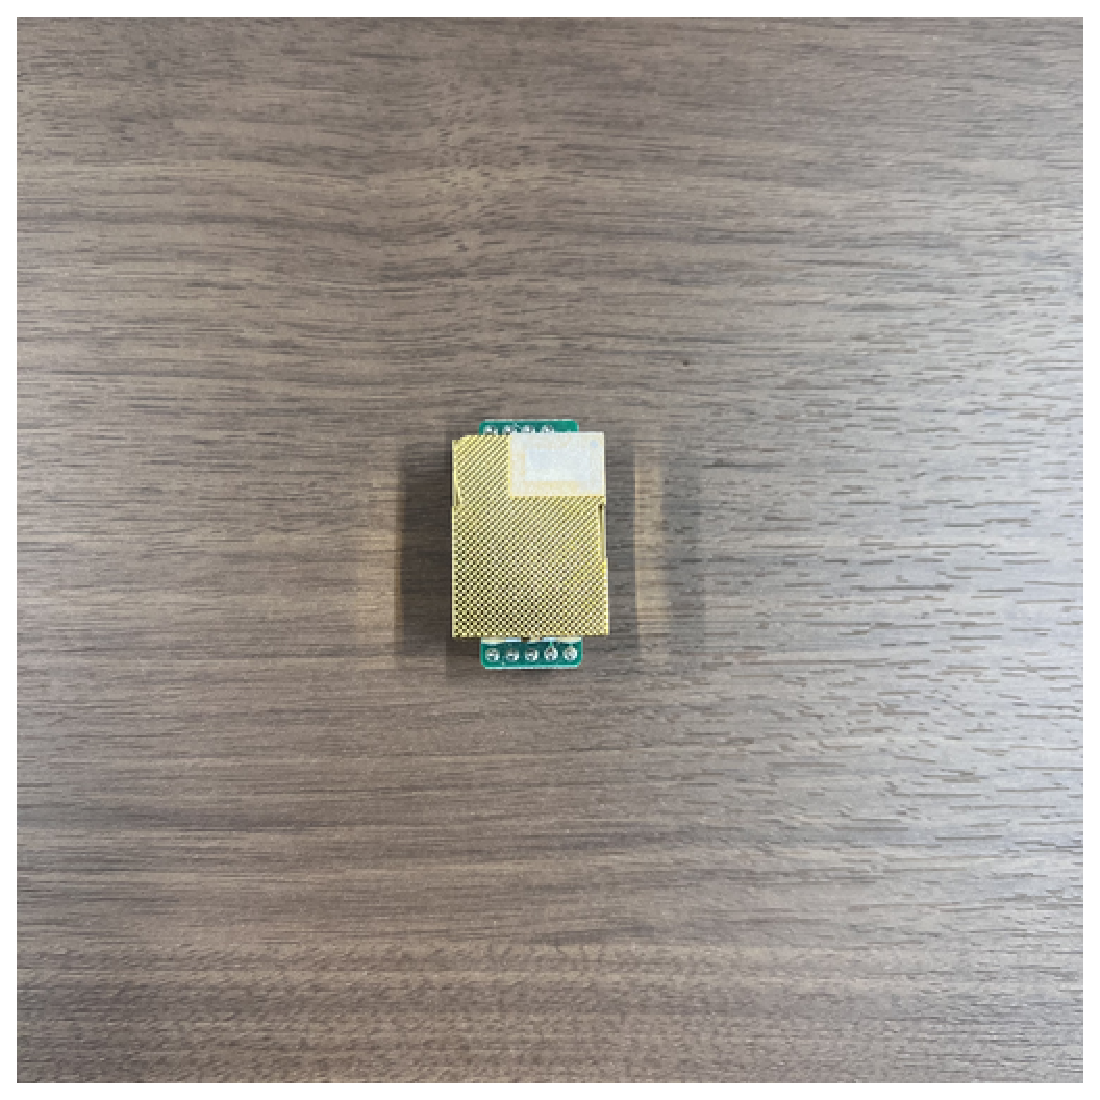
\includegraphics[width=\linewidth]{./figures/mh-z19c}
  \captionof{figure}{MH-Z19C}
  \label{fig:mh-z19c}
\end{minipage}
\hfill
\begin{minipage}{0.52\linewidth}
  \centering
  \captionof{table}{MH-Z19Cの主なパラメータ}
  \label{tab:mhz19cParameters}
  \begin{tabular}{|c|c|}
    \hline
    項目 & 内容 \\ \hline \hline
    測定方式 & NDIR \\ \hline
    CO$_2$測定範囲 & 0$\sim$5000 ppm \\ \hline
    測定精度 & $\pm$(50 ppm + 5\%) \\ \hline
    応答時間 & $<$120 s \\ \hline
    動作電圧 & 4.5$\sim$5.5 V \\ \hline
    平均消費電流 & 約60 mA \\ \hline
    通信方式 & UART / PWM \\ \hline
    用途 & 室内据え置き測定 \\ \hline
  \end{tabular}
\end{minipage}

\end{figure}
\FloatBarrier


\subsection{温度・湿度・気圧センサ BME680}
BME680 は,Bosch Sensortec 社製の環境センサであり,温度,湿度,気圧に加えてガスセンサを内蔵している。内蔵されたガスセンサは主に揮発性有機化合物(VOC)に反応し,室内空気中の汚染度を間接的に評価することが可能である。先行研究では,これら複数の環境指標を組み合わせることで,室内環境を総合的に評価する目的で本センサが使用されていた。本モジュールの主なパラメータを表\ref{tab:bme680Parameters}に示す。

\begin{figure}[H]
\centering

\begin{minipage}{0.42\linewidth}
  \centering
  \includegraphics[width=\linewidth]{./figures/bme}
  \captionof{figure}{BME680}
  \label{fig:BME680}
\end{minipage}
\hfill
\begin{minipage}{0.52\linewidth}
  \centering
  \captionof{table}{BME680の主なパラメータ}
  \label{tab:bme680Parameters}
  \begin{tabular}{|c|c|}
    \hline
    項目 & 内容 \\ \hline \hline
    測定対象 & 温度・湿度・気圧・VOC \\ \hline
    通信方式 & I$^2$C / SPI \\ \hline
    動作電圧 & 1.7$\sim$3.6 V \\ \hline
    用途 & 環境モニタリング \\ \hline
  \end{tabular}
\end{minipage}

\end{figure}
\FloatBarrier

\section{開発環境}
本研究におけるソフトウェア開発には Arduino IDE を使用した。Arduino IDE は,マイクロコントローラ向けの統合開発環境であり,プログラムの作成,コンパイル,書き込みを一貫して行うことができる。本研究では Arduino IDE Version 2.3.7 を使用し,ESP32-C6 および各種センサ,通信モジュールの制御プログラムを開発した。また,Arduino CLI Version 1.3.1 が内部的に用いられており,ビルドおよび書き込み処理が行われている。
